\newpage
\section{Bola, Para Bola}           
\begin{teachingnote}
A major purpose here is to explain, from the geometry and also from the algebra, the form of the result:
$y = ax^2 + bx + c$ or $x = ay^2 + by + c$.  
\end{teachingnote}
We've mentioned several times that a parabola is the set of points
that are equidistant from a given point (the focus) and a given line
(the directrix):\index{focus}\index{directrix}
\[
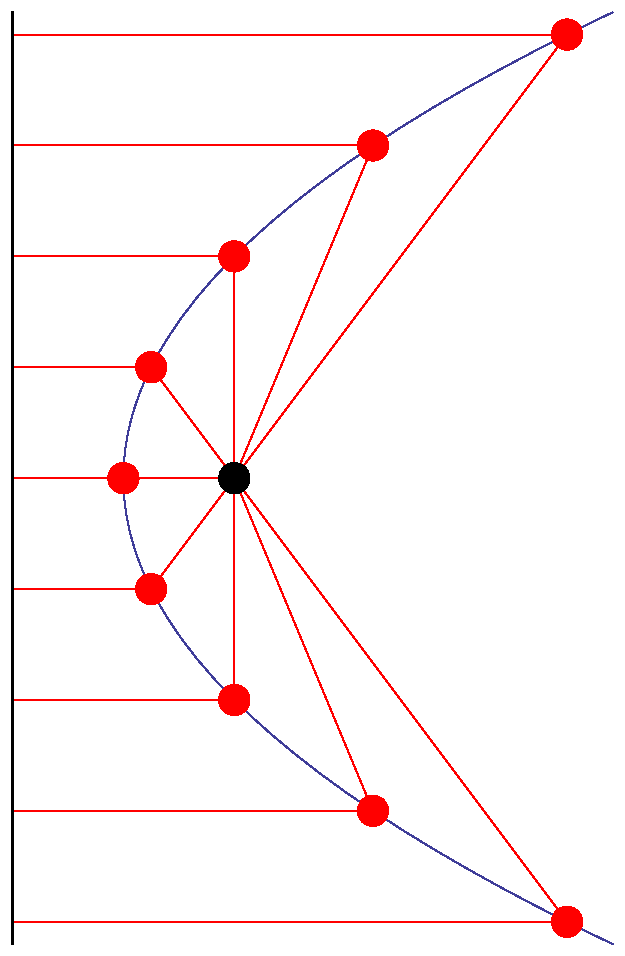
\includegraphics[angle=90,scale=.35]{../graphics/parabolapointline.pdf}
\]
In this activity we are going to reconcile the definition given
above with the equation that you know and love (admit it!):
\[
y = ax^2 + bx + c
\]

\begin{prob}
How do we compute the distance between two points? Be explicit!
\end{prob}

\begin{prob}
Let's see if we can derive the formula for a parabola with its focus at $(0,1)$ and its directrix being the line $y=0$.
\begin{enumerate}
\item Graph the focus and the directrix, sketch what the parabola might look like, and identify a generic point $(x, y)$.  
\item Draw on the graph the distance from $(x,y)$ to the focus.  Write an expression for this distance.  
\item Draw on the graph the distance from $(x,y)$ to the directrix.  Write an expression for this distance.  
\item Use these two expressions and some algebra to find the formula for the parabola. 
\vspace{.5in}
\item How might you have known, before completing the algebra, that the result would be in the form 
$y = ax^2 + bx + c$? 
\end{enumerate}
\end{prob}
\vspace{.5in}

\begin{prob}
Now derive the formula for a parabola with focus at $(2,1)$ and directrix $y=-1$.
\end{prob}
\vspace{1in}

\begin{prob}
Now derive the formula for a parabola with focus at $(1,-3)$ and directrix $x=3$.  How might you have known, before completing the algebra, the form of the result?   
\end{prob}





